\section{Preisstabilität}
\vspace{-0.5cm}
\begin{minipage}{0.5\linewidth}
    \subsection{Inflation}
    Eine Inflation bedeutet eine permanente Steigerung des Preisniveaus.\\
    Auslöser ist eine einmalige Steigerung des Preisniveaus durch einen positiven Nachfrageschock oder einen negativen Angebotsschock. Ob dies zu einer Inflation führt hängt von der Inflationserwartung der Haushalte und Unternehmen ab. Bei einer Erhöhung der Geldmenge sinkt der Zinssatz und gleichzeitig steigt die Nachfrage nach Geld. 
\end{minipage}
\begin{minipage}{0.5\linewidth}
    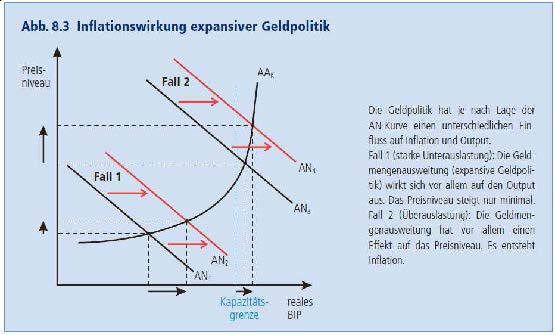
\includegraphics[width=\linewidth]{images/Inflationswirkung}
\end{minipage}
\vspace{-1cm}
\subsubsection{Lohn-Preis-Spirale}
Erhöhtes Preisniveau durch einmaligen Schock.
\begin{itemize}
	\item 1. Sinkende Reallöhne der Haushalte
	\item 2. Diese fordern (Inflationserwartung) eine Steigerung der Nominallöhne, welche die Erhöhung des Preisniveau überkompensiert
	\item 3. Damit ergbit sich eine Steigerung der Reallöhne
	\item 4. Dies bedeutet für die Unternehmen eine Kostensteigerung
	\item 5. Die Unternehmen werden deshalb höhere Güterpreise verlangen
	\item 6. Damit erhöht sich wieder das Preisniveau (Zweitrundeneffekt)
	\item Retour zu 1.
\end{itemize}
Die Inflation funktioniert nur, wenn die Nationalbank mitspielt und Geld druckt. Erwarten die Haushalte keine Steigerung setzt sich die Spirale nicht in Bewegung. Hinter jeder Inflation ist eine Vergrösserung der Geldmenge, welche grösser ist als der Zuwachs des realen BIP. 
\vspace{-0.5cm}
\subsubsection{Quantitätsgleichung}
\vspace{-1cm}
\begin{align*} 
    P \cdot Q &= M \cdot V\\
	\underbrace{Preisniveau \cdot reales \; BIP}_{\text nomiales \; BIP} &= Geldmenge \cdot Geldumlaufgeschwindigkeit
\end{align*}
\subsubsection{Kosten der Inflation}
\begin{itemize}
	\item Viele kleine Bankabhebungen (Transaktionskosten)
	\item Kosten der Unsicherheit (Zinsen)
	\item Kosten aufgrund der Verzerrung der relativen Preise
	\item Kosten für Kreditgeber, Inflation frisst Zins auf
	\item Kosten aufgrund höheres Nominaleinkommen, mehr Steuern
	\item Inflation wird mit Verkleinerung der Geldmenge bekämpft, dadurch oftmals Rezession
\end{itemize}
\subsection{Deflation}
Eine Deflation bedeutet ein permanenter Rückgang des Preisniveau. 
Die Deflation ist dann schädlich wenn diese auf einem Rückgang der aggregierten Nachfrage beruht. Ein Preisrückgang aufgrund einer Ausweitung des aggregierten Angebots führt zu keiner Deflation. Die Deflation ist kaum durch Geldpolitik und Fiskalpolitik zu lösen, weil alle erwarten dass es günstiger wird, daher hat die Ausweitung der Geldmenge keinen Effekt.
\vspace{-0.5cm}
\subsubsection{Folgen der Deflation}
\begin{itemize}
    \item Selbstverstärkende Wirkung
    \subitem Ausgelöst durch ausgeprägte Deflationserwartungen
    \item Hohe Realzinsen
    \subitem Realzins = Nominalzins (minimal 0\%) + erwartete Deflation
    \item Steigende Reallöhne
    \subitem Steigende Produktionskosten für Unternehmen
    \item Sinkende Bonität der Schuldner und Bankkrisen
    \subitem Kreditgeber gewinnen (Haushalte), Kreditnehmer verlieren
    (steigender Realwert der Schulden)
\end{itemize}

\clearpage
\pagebreak